% Propósito: comparar la refracción por dos perfiles térmicos opuestos.
% Origen: c(z) depende de la temperatura; los rayos se curvan hacia la
% región de menor velocidad. Esquema cualitativo, sin datos experimentales.
% Accesibilidad: dos paneles muestran suelo cálido con curvatura ascendente
% y una inversión térmica con curvatura descendente.
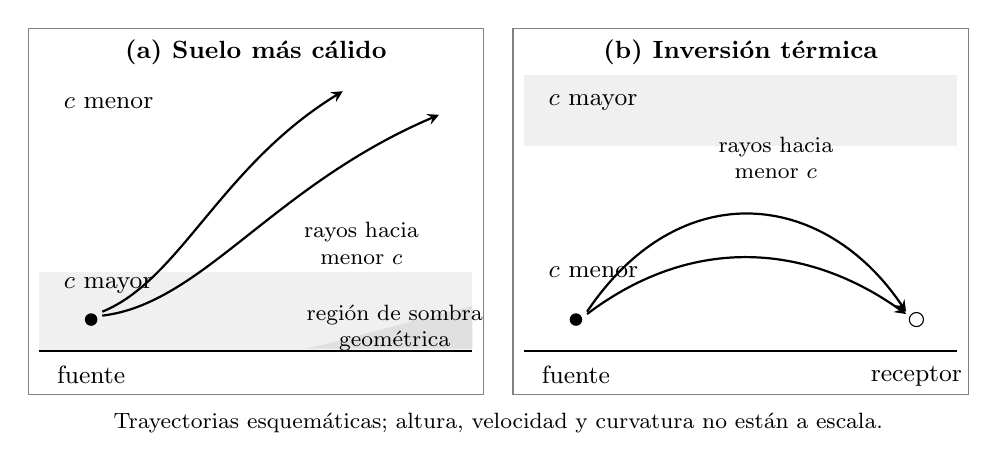
\begin{tikzpicture}[
    x=0.94cm,
    y=1cm,
    >=stealth,
    font=\small,
    rayo/.style={thick,->},
    guia/.style={gray,dashed},
    banda/.style={fill=black!6,draw=none}
]
    % Panel diurno
    \draw[gray] (0,0) rectangle (6.15,4.65);
    \node[font=\small\bfseries] at (3.075,4.35) {(a) Suelo más cálido};
    \path[banda] (0.15,0.55) rectangle (6.0,1.55);
    \draw[thick] (0.15,0.55) -- (6.0,0.55);
    \node[anchor=west] at (0.35,1.38) {\(c\) mayor};
    \node[anchor=west] at (0.35,3.70) {\(c\) menor};
    \node[fill=black,circle,inner sep=1.6pt] (sd) at (0.85,0.95) {};
    \node[anchor=north] at (0.85,0.48) {fuente};
    \draw[rayo] (1.0,1.00)
        .. controls (2.35,1.15) and (3.30,2.65) .. (5.55,3.55);
    \draw[rayo] (1.0,1.05)
        .. controls (2.05,1.45) and (2.60,2.90) .. (4.25,3.85);
    \path[fill=black!12] (3.75,0.58) -- (6.0,0.58) -- (6.0,1.12)
        .. controls (5.1,0.92) and (4.45,0.73) .. cycle;
    \node[align=center,font=\footnotesize] at (4.95,0.84)
        {región de sombra\\geométrica};
    \node[align=center,font=\footnotesize] at (4.50,1.92)
        {rayos hacia\\menor \(c\)};

    % Panel con inversión
    \draw[gray] (6.55,0) rectangle (12.70,4.65);
    \node[font=\small\bfseries] at (9.625,4.35) {(b) Inversión térmica};
    \path[banda] (6.70,3.15) rectangle (12.55,4.05);
    \draw[thick] (6.70,0.55) -- (12.55,0.55);
    \node[anchor=west] at (6.90,1.55) {\(c\) menor};
    \node[anchor=west] at (6.90,3.70) {\(c\) mayor};
    \node[fill=black,circle,inner sep=1.6pt] (sn) at (7.40,0.95) {};
    \node[anchor=north] at (7.40,0.48) {fuente};
    \node[draw,circle,inner sep=1.8pt] (rn) at (12.0,0.95) {};
    \node[anchor=north] at (12.0,0.48) {receptor};
    \draw[rayo] (7.55,1.05)
        .. controls (8.80,2.80) and (10.75,2.60) .. (11.86,1.05);
    \draw[rayo] (7.55,1.02)
        .. controls (9.00,2.05) and (10.55,1.90) .. (11.86,1.02);
    \node[align=center,font=\footnotesize] at (10.10,3.00)
        {rayos hacia\\menor \(c\)};

    \node[font=\footnotesize,anchor=north] at (6.35,-0.12)
        {Trayectorias esquemáticas; altura, velocidad y curvatura no están a escala.};
\end{tikzpicture}
